\documentclass[11pt]{article}
\usepackage{amsmath,amssymb,amsmath,amsthm,amsfonts}
\usepackage{latexsym,graphicx}
\usepackage{fullpage,color}
\usepackage{url}
\usepackage[pdftex,bookmarks,colorlinks=true,citecolor=blue]{hyperref}
\usepackage{natbib}
\usepackage{graphicx,subfigure}
\usepackage{algorithm}
\usepackage{algorithmic}
\usepackage{listings}
\usepackage{xcolor}
\usepackage{framed}
\usepackage{color}
\usepackage{titlesec}


\titleformat{\subsubsection}[runin]{\bfseries}{}{}{}[]

% \colorlet{shadecolor}{orange!15}
\colorlet{NextBlue}{orange!15!green!50!blue!75}

\numberwithin{equation}{section}

\pagestyle{plain}

\setlength{\oddsidemargin}{0in}
\setlength{\topmargin}{0in}
\setlength{\textwidth}{6.5in}
\setlength{\textheight}{8.5in}

\newtheorem{fact}{Fact}[section]
\newtheorem{question}{Question}[section]
\newtheorem{lemma}{Lemma}[section]
\newtheorem{theorem}[lemma]{Theorem}
\newtheorem{assumption}[lemma]{Assumption}
\newtheorem{corollary}[lemma]{Corollary}
\newtheorem{prop}[lemma]{Proposition}
\newtheorem{claim}{Claim}[section]
\newtheorem{remark}{Remark}[section]
\newtheorem{definition}{Definition}[section]
\newtheorem{prob}{Problem}[section]
\newtheorem{conjecture}{Conjecture}[section]
\newtheorem{property}{Property}[section]

\def\A{{\bf A}}
\def\a{{\bf a}}
\def\B{{\bf B}}
\def\bb{{\bf b}}
\def\C{{\bf C}}
\def\c{{\bf c}}
\def\D{{\bf D}}
\def\d{{\bf d}}
\def\E{{\bf E}}
\def\e{{\bf e}}
\def\F{{\bf F}}
\def\f{{\bf f}}
\def\g{{\bf g}}
\def\h{{\bf h}}
\def\G{{\bf G}}
\def\H{{\bf H}}
\def\I{{\bf I}}
\def\K{{\bf K}}
\def\k{{\bf k}}
\def\LL{{\bf L}}
\def\M{{\bf M}}
\def\m{{\bf m}}
\def\N{{\bf N}}
\def\n{{\bf n}}
\def\PP{{\bf P}}
\def\pp{{\bf p}}
\def\Q{{\bf Q}}
\def\q{{\bf q}}
\def\R{{\bf R}}
\def\rr{{\bf r}}
\def\S{{\bf S}}
\def\s{{\bf s}}
\def\T{{\bf T}}
\def\tt{{\bf t}}
\def\U{{\bf U}}
\def\u{{\bf u}}
\def\V{{\bf V}}
\def\v{{\bf v}}
\def\W{{\bf W}}
\def\w{{\bf w}}
\def\X{{\bf X}}
\def\x{{\bf x}}
\def\Y{{\bf Y}}
\def\y{{\bf y}}
\def\Z{{\bf Z}}
\def\z{{\bf z}}
\def\0{{\bf 0}}
\def\1{{\bf 1}}



\def\AM{{\mathcal A}}
\def\CM{{\mathcal C}}
\def\DM{{\mathcal D}}
\def\EM{{\mathcal E}}
\def\GM{{\mathcal G}}
\def\FM{{\mathcal F}}
\def\IM{{\mathcal I}}
\def\JM{{\mathcal J}}
\def\KM{{\mathcal K}}
\def\LM{{\mathcal L}}
\def\NM{{\mathcal N}}
\def\OM{{\mathcal O}}
\def\PM{{\mathcal P}}
\def\SM{{\mathcal S}}
\def\TM{{\mathcal T}}
\def\UM{{\mathcal U}}
\def\VM{{\mathcal V}}
\def\WM{{\mathcal W}}
\def\XM{{\mathcal X}}
\def\YM{{\mathcal Y}}
\def\RB{{\mathbb R}}
\def\RBmn{{\RB^{m\times n}}}
\def\EB{{\mathbb E}}
\def\PB{{\mathbb P}}

\def\TX{\tilde{\bf X}}
\def\TA{\tilde{\bf A}}
\def\tx{\tilde{\bf x}}
\def\ty{\tilde{\bf y}}
\def\TZ{\tilde{\bf Z}}
\def\tz{\tilde{\bf z}}
\def\hd{\hat{d}}
\def\HD{\hat{\bf D}}
\def\hx{\hat{\bf x}}
\def\nysA{{\tilde{\A}_c^{\textrm{nys}}}}

\def\alp{\mbox{\boldmath$\alpha$\unboldmath}}
\def\bet{\mbox{\boldmath$\beta$\unboldmath}}
\def\epsi{\mbox{\boldmath$\epsilon$\unboldmath}}
\def\etab{\mbox{\boldmath$\eta$\unboldmath}}
\def\ph{\mbox{\boldmath$\phi$\unboldmath}}
\def\pii{\mbox{\boldmath$\pi$\unboldmath}}
\def\Ph{\mbox{\boldmath$\Phi$\unboldmath}}
\def\Ps{\mbox{\boldmath$\Psi$\unboldmath}}
\def\ps{\mbox{\boldmath$\psi$\unboldmath}}
\def\tha{\mbox{\boldmath$\theta$\unboldmath}}
\def\Tha{\mbox{\boldmath$\Theta$\unboldmath}}
\def\muu{\mbox{\boldmath$\mu$\unboldmath}}
\def\Si{\mbox{\boldmath$\Sigma$\unboldmath}}
\def\si{\mbox{\boldmath$\sigma$\unboldmath}}
\def\Gam{\mbox{\boldmath$\Gamma$\unboldmath}}
\def\Lam{\mbox{\boldmath$\Lambda$\unboldmath}}
\def\De{\mbox{\boldmath$\Delta$\unboldmath}}
\def\Ome{\mbox{\boldmath$\Omega$\unboldmath}}
\def\Pii{\mbox{\boldmath$\Pi$\unboldmath}}
\def\varepsi{\mbox{\boldmath$\varepsilon$\unboldmath}}
\newcommand{\ti}[1]{\tilde{#1}}
\def\Ncal{\mathcal{N}}
\def\argmax{\mathop{\rm argmax}}
\def\argmin{\mathop{\rm argmin}}

\def\ALG{{\AM_{\textrm{col}}}}

\def\mean{\mathsf{mean}}
\def\std{\mathsf{std}}
\def\bias{\mathsf{bias}}
\def\var{\mathsf{var}}
\def\sgn{\mathsf{sgn}}
\def\tr{\mathsf{tr}}
\def\rk{\mathrm{rank}}
\def\nnz{\mathsf{nnz}}
\def\poly{\mathrm{poly}}
\def\diag{\mathsf{diag}}
\def\Diag{\mathsf{Diag}}
\def\const{\mathrm{Const}}
\def\st{\mathsf{s.t.}}
\def\vect{\mathsf{vec}}
\def\sech{\mathrm{sech}}
\def\sigmoid{\mathsf{sigmoid}}

\newcommand{\red}[1]{{\color{red}#1}}



\def\argmax{\mathop{\rm argmax}}
\def\argmin{\mathop{\rm argmin}}

\newenvironment{note}[1]{\medskip\noindent \textbf{#1:}}%
        {\medskip}


\newcommand{\etal}{{\em et al.}\ }
\newcommand{\assign}{\leftarrow}
\newcommand{\eps}{\epsilon}

\newcommand{\opt}{\textrm{\sc OPT}}
\newcommand{\script}[1]{\mathcal{#1}}
\newcommand{\ceil}[1]{\lceil #1 \rceil}
\newcommand{\floor}[1]{\lfloor #1 \rfloor}



\lstset{ %
extendedchars=false,            % Shutdown no-ASCII compatible
language=Python,                % choose the language of the code
xleftmargin=1em,
xrightmargin=1em,
basicstyle=\footnotesize,    % the size of the fonts that are used for the code
tabsize=3,                            % sets default tabsize to 3 spaces
numbers=left,                   % where to put the line-numbers
numberstyle=\tiny,              % the size of the fonts that are used for the line-numbers
stepnumber=1,                   % the step between two line-numbers. If it's 1 each line
                                % will be numbered
numbersep=5pt,                  % how far the line-numbers are from the code   %
keywordstyle=\color[rgb]{0,0,1},                % keywords
commentstyle=\color[rgb]{0.133,0.545,0.133},    % comments
stringstyle=\color[rgb]{0.627,0.126,0.941},      % strings
backgroundcolor=\color{white}, % choose the background color. You must add \usepackage{color}
showspaces=false,               % show spaces adding particular underscores
showstringspaces=false,         % underline spaces within strings
showtabs=false,                 % show tabs within strings adding particular underscores
frame=single,                 % adds a frame around the code
%captionpos=b,                   % sets the caption-position to bottom
breaklines=true,                % sets automatic line breaking
breakatwhitespace=false,        % sets if automatic breaks should only happen at whitespace
%title=\lstname,                 % show the filename of files included with \lstinputlisting;
%                                % also try caption instead of title
mathescape=true,escapechar=?    % escape to latex with ?..?
escapeinside={\%*}{*)},         % if you want to add a comment within your code
%columns=fixed,                  % nice spacing
%morestring=[m]',                % strings
%morekeywords={%,...},%          % if you want to add more keywords to the set
%    break,case,catch,continue,elseif,else,end,for,function,global,%
%    if,otherwise,persistent,return,switch,try,while,...},%
}


\begin{document}

%\setlength{\fboxrule}{.5mm}\setlength{\fboxsep}{1.2mm}
%\newlength{\boxlength}\setlength{\boxlength}{\textwidth}
%\addtolength{\boxlength}{-4mm}


\title{Hacking Smart Machines with Smarter Ones: How to Extract Meaningful Data from Machine Learning Classifiers}

\author{\textbf{Giuseppe Ateniese\etal}}

%\date{ }

\maketitle

\begin{abstract}
% This lecture note describes synchronous parallel accelerated gradient descent (AGD) for empirical risk minimization ERM.
% We first describe AGD for solving ERM.
% We then show how to parallelize AGD; in particular, we assume there is a central parameter server and the data are partitioned among the worker nodes.
% We finally use Python to write a simulator that mimics synchronous parallel AGD.
This paper focuses on ML classifiers and the statistical information that can be unconsciously or maliciously revealed from them. They show that it is possible to infer unexpected but useful information from ML classifiers.
https://www.overleaf.com/project/5dce27a482b81a0001f5883a
\end{abstract}

\section{Motivation: Is it safe to release a profitable ML classifier?} 

\subsubsection*{Example: }a classifier $C_a$ is less effective than a classifier $C_b$.

$C_b$: publicly available or can be inferred through reverse engineering. 

We could assume that the training set used for $C_b$ is \textit{superior}, in the sense that makes $C_b$ more effective than $C_b$ even though both implement essentially the same ML algorithm.

\subsubsection*{Question:}~

Would a classifier reveal concrete hints about its training set?
\subsubsection*{Answer:}~

A classifier is possible to extract meaningful information about its training set.

\subsubsection*{Reason:}~

A typical ML classifier learns by changing its internal structure to absorb the information contained in the training data.

\subsubsection*{Model they proposed:}~

a meta-classifier, to detect and classify these changes and deduce valuable information

\subsubsection*{\color{red}Important points}

It is important to observe that we are not interested in privacy leaks, but rather in discovering anything that makes classifiers better than others. 

\textbf{e.g., a speech recognition software recognizes spoken words better than competing products, even though they all implement the same ML algorithms}

\textbf{training set:} commonly spoken words(does not make sense to talk about privacy protection)

\textbf{meta-classifier to reveal:} the majority of training samples came from female voices or from voices of people with marked accents (e.g., Indian, British, American, etc.)

Possibly uncovering the secret sauce makes the speech recognition software stay ahead of the competition.

\section{Contributions}

\begin{itemize}
    \item a new type of information leakage
    \item devise a general attack strategy, using a meta-classifier to extract meaningful data from the target classifier.
    \item successfully attack some existing ML classifiers.(SVMs, HMMs)
\end{itemize}


\section{An attack strategy}

\begin{figure}[H]
    \centering
    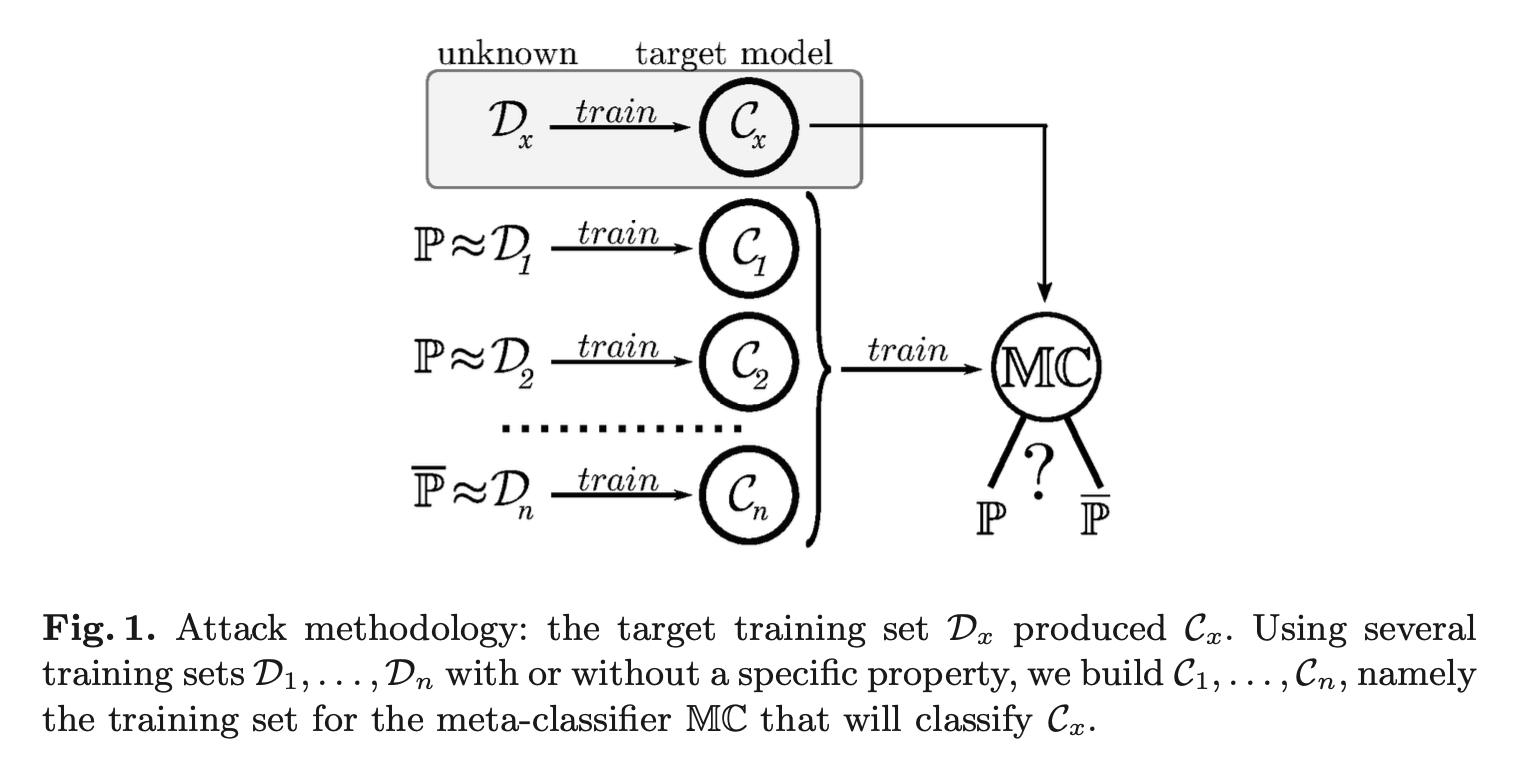
\includegraphics[width = 15cm]{figures/Attack_methodology.png}
    % \caption{Caption}
    \label{fig:my_label}
\end{figure}

\textbf{Remark:} With this methodology the adversary extracts \textit{external information}, NOT in the form of attributes of the dataset $D_x$.

They also use some \textit{filters} to improve the performance of meta-classifier.

\textbf{Experiment1:HMM for speech recognition}

\textbf{property $P$:} the classifier was trained only with people who speak an Indian english dialect

meta-classifier: decision tree

\begin{figure}[H]
    \centering
    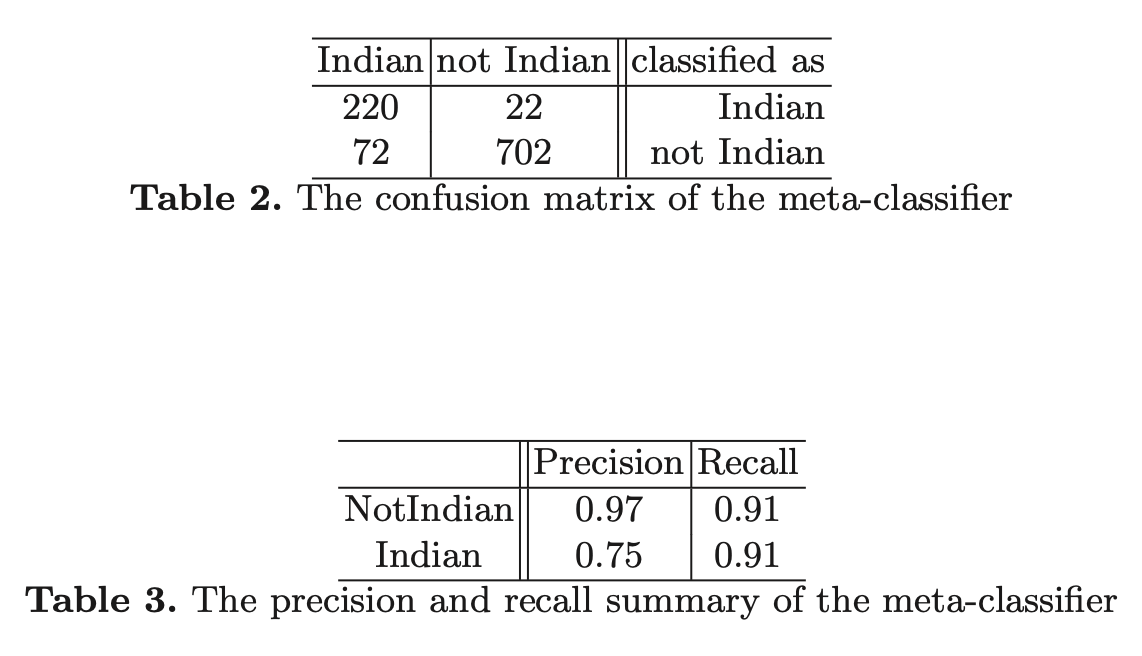
\includegraphics[width = 15cm]{figures/e1_non_filtered.png}
    % \caption{Caption}  
    \label{fig:my_label}
\end{figure}

\begin{figure}[H]
    \centering
    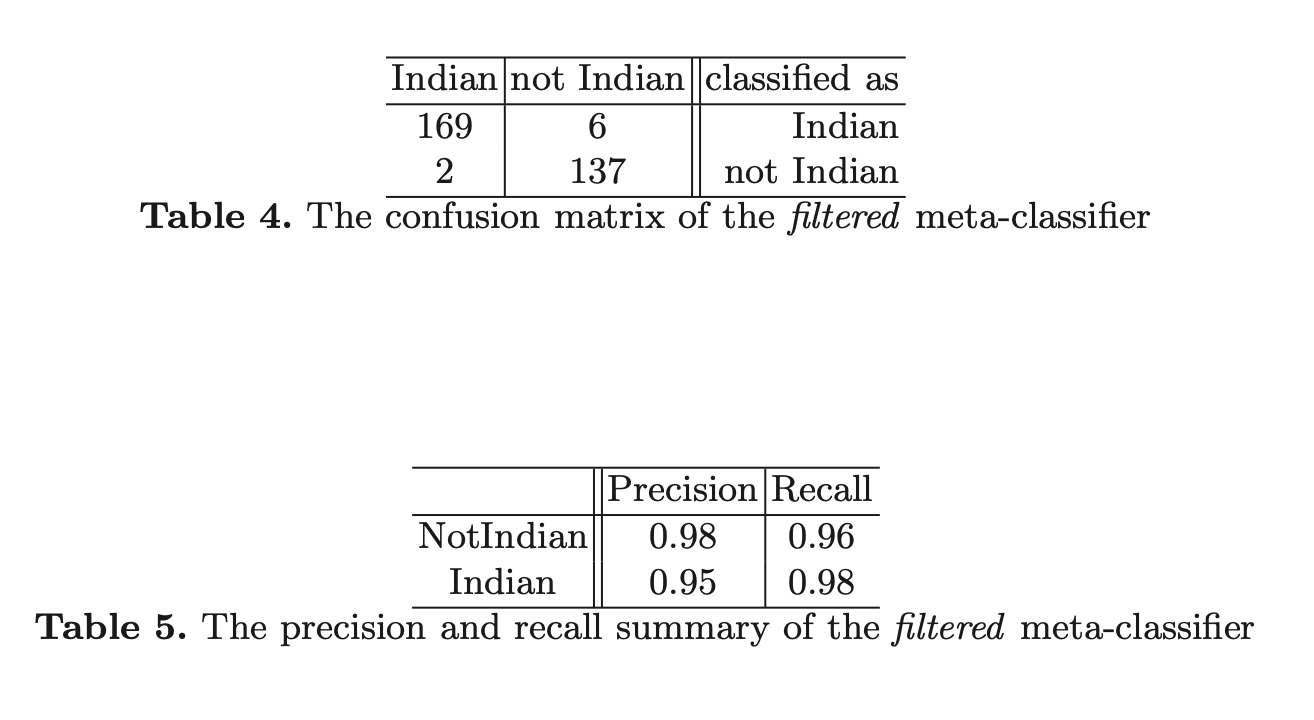
\includegraphics[width = 15cm]{figures/e1_filtered.png}
    % \caption{Caption}  /
    \label{fig:my_label}
\end{figure}

\textbf{Experiment1:SVM for network traffic classification}

\textbf{extrapolate the type of traffic:} whether Google web traffic was used in the training samples?

\begin{figure}[H]
    \centering
    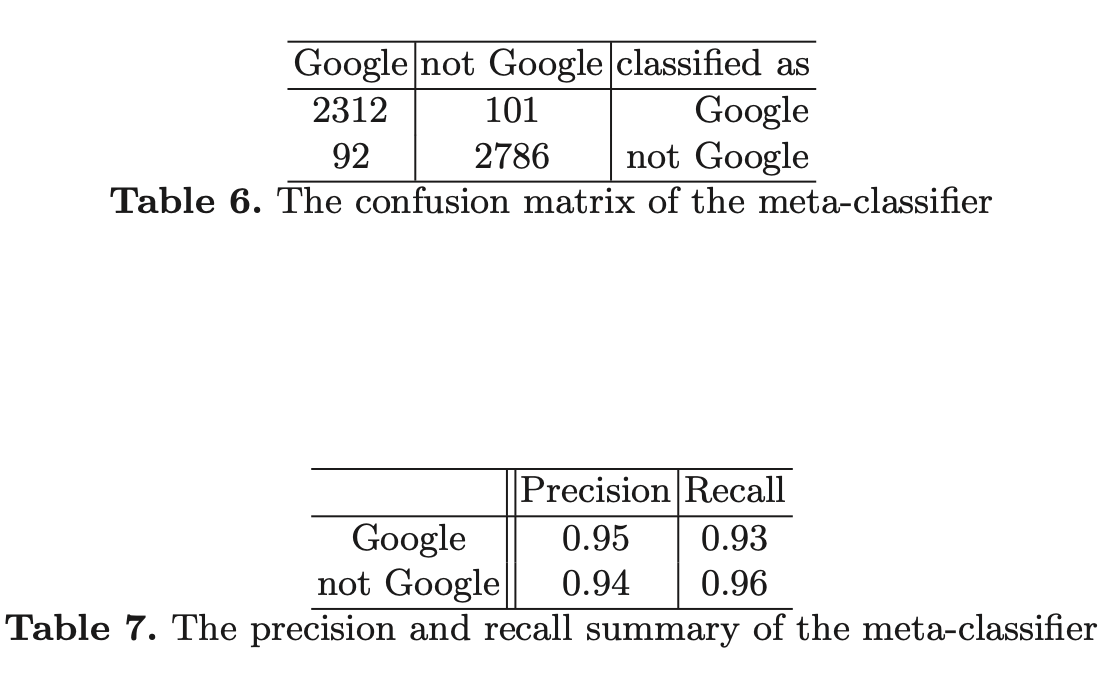
\includegraphics[width = 15cm]{figures/google.png}
    % \caption{Caption}  /
    \label{fig:my_label}
\end{figure}

\textbf{Result: }we were able to build an effective meta-classifier that infers whether the training set given as input includes also a specific type of traffic.


\textbf{Experiment1:Hacking models secured by Differential Privacy}

Differential privacy is ineffective against this attack strategy.

\begin{enumerate}
    \item obfuscate the original database D and transform it into $D^{\prime}$. {\color{blue}The adversary is not interested in D, it is eager for any information on $D^{\prime}$}
    \item train a classifier and then add noise to the output. {\color{blue}adversary has complete access to the classifier}
    \item adding noise during training, thus effectively obfuscating the learning process.{\color{blue}the final classifier must anyway converge to classify correctly the training set.}
\end{enumerate}


\begin{figure}[H]
    \centering
    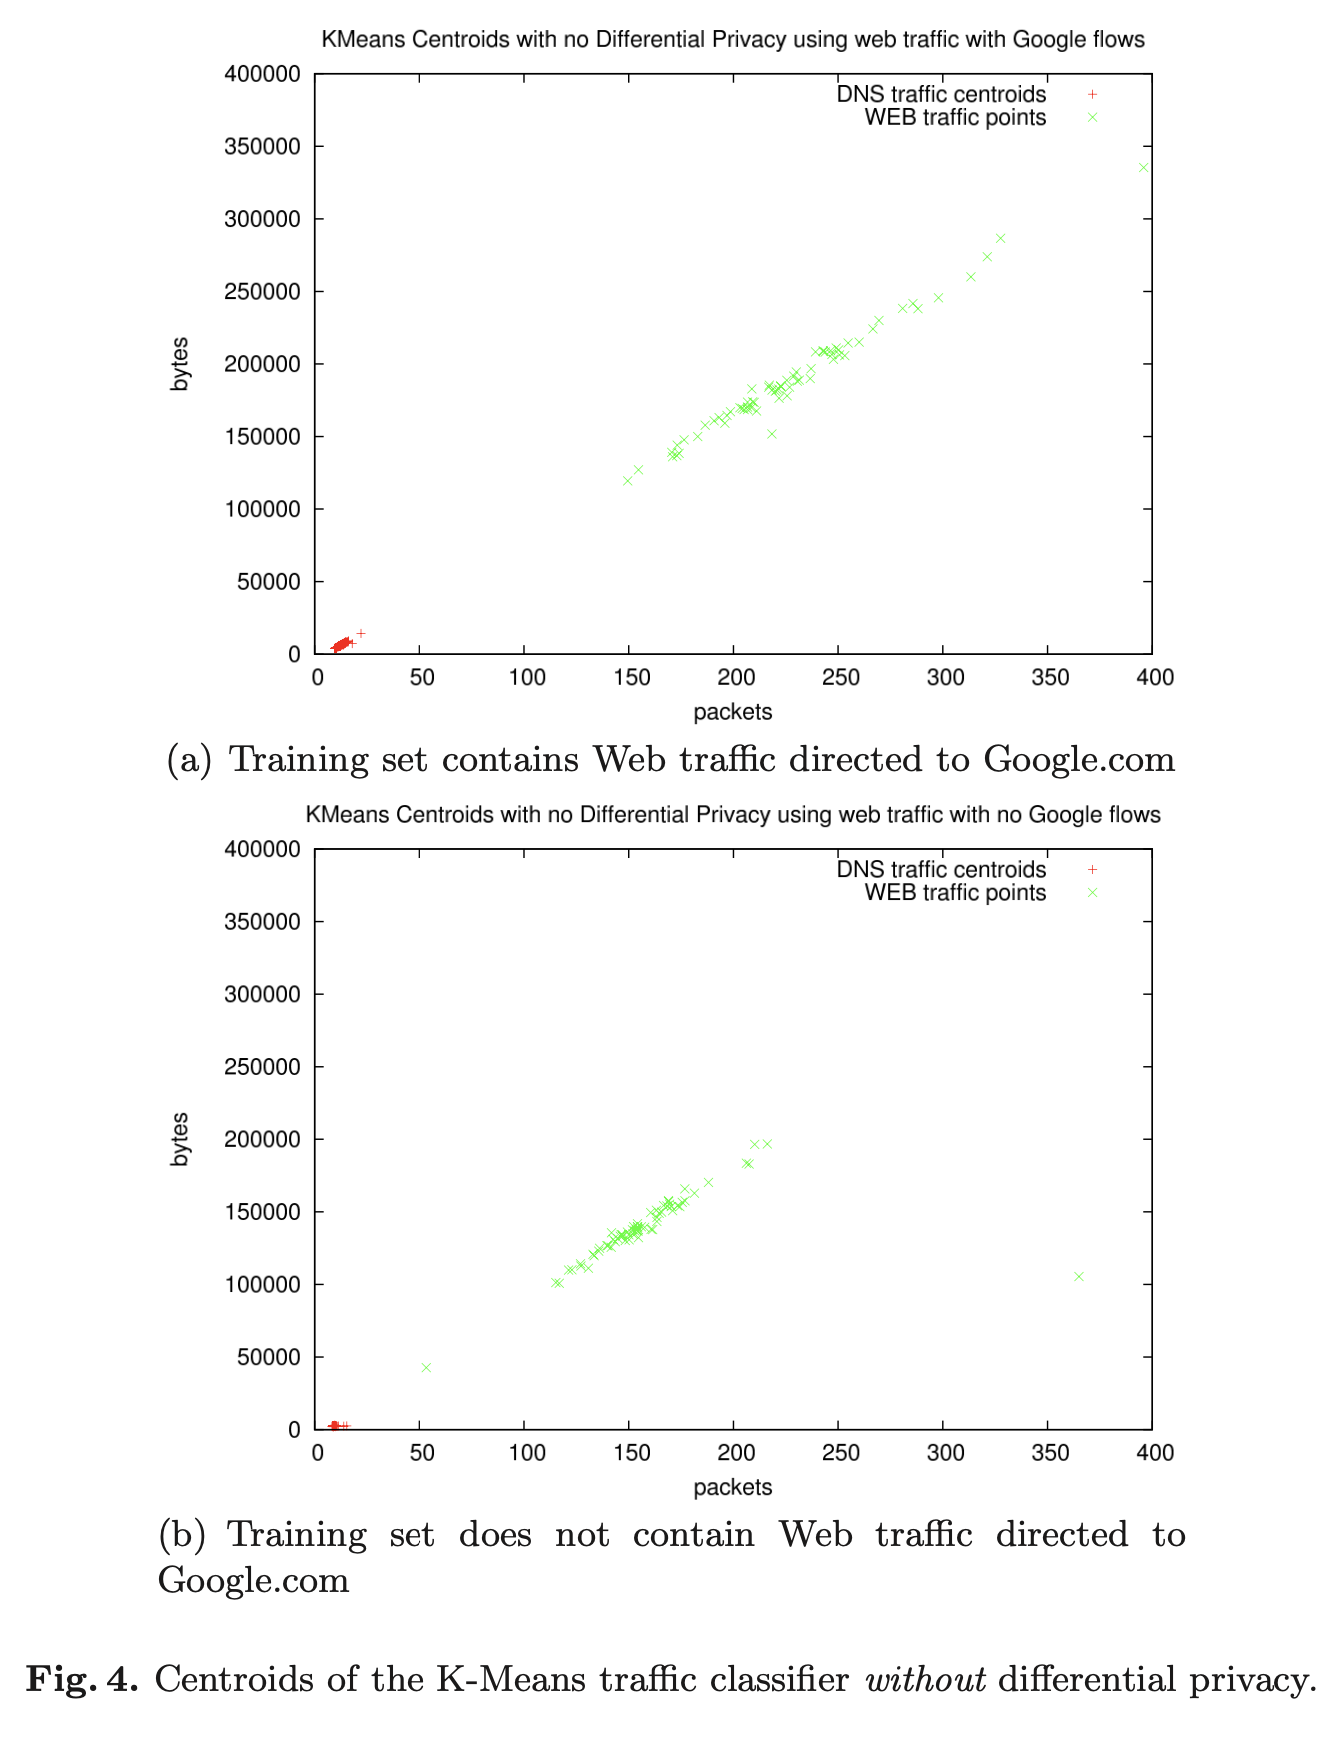
\includegraphics[width = 15cm]{figures/google_non_diff.png}
    % \caption{Caption}  /
    \label{fig:my_label}
\end{figure}

 The pictures represent the centroids when there is traffic to Google.com and no traffic to Google.com in figure. It is easy to see that the positions of the centroids are quite different, allowing us to easily distinguish between these two cases.

\begin{figure}[H]
    \centering
    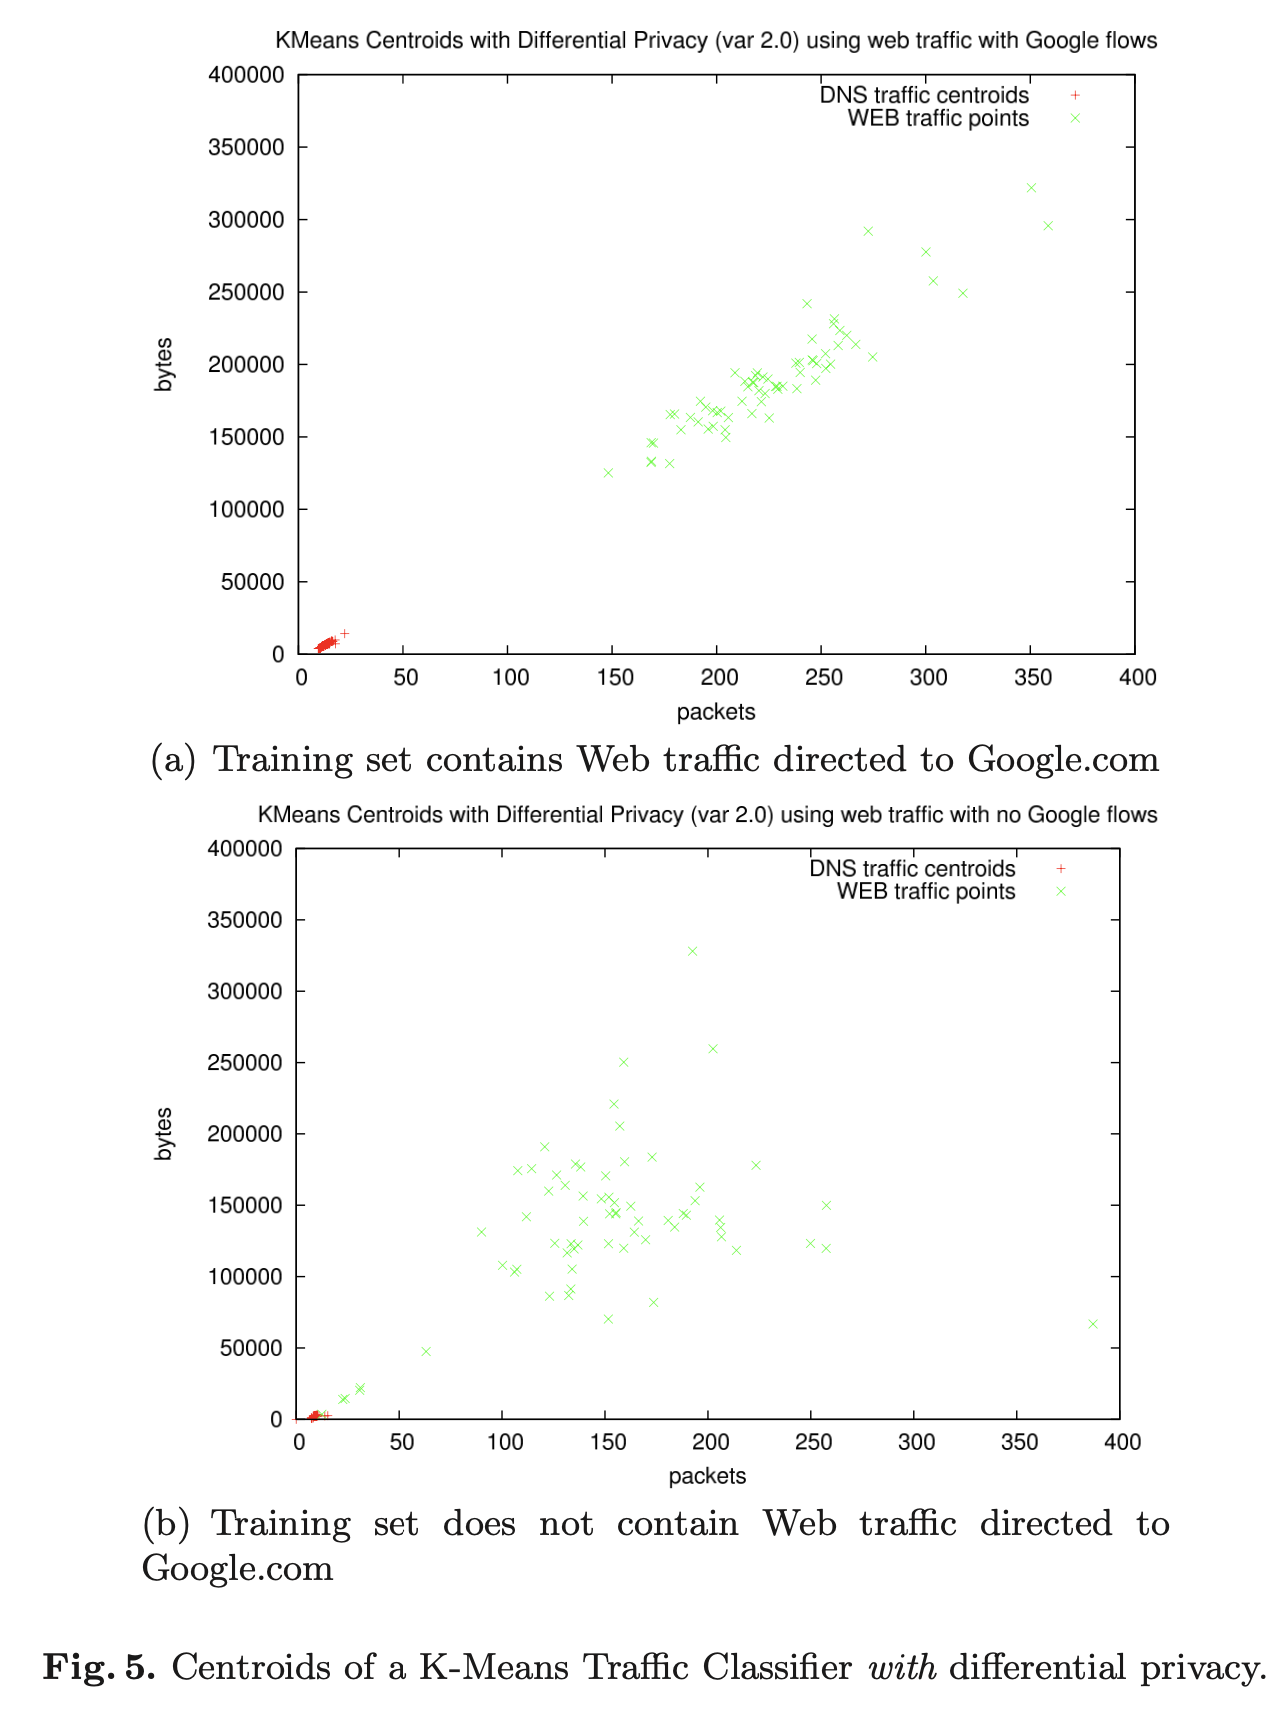
\includegraphics[width = 14cm]{figures/google_diff.png}
    % \caption{Caption}  /
    \label{fig:my_label}
\end{figure}
Similar results appear when we picture the centroids of the classifier providing differential privacy. An adversary can easily distinguish whether there is Google.com traffic or not.


% \bibliographystyle{plain}

% %\markboth{\bibname}{\bibname}
% % \bibliography{bib/decentralized,bib/distributed,bib/system}
% \bibliography{bib/decentralized,bib/distributed,bib/system,bib/poison}

\end{document}
